\documentclass[10pt,a4paper]{article}

% --- Essential Packages ---
\usepackage[utf8]{inputenc}
\usepackage[T1]{fontenc}
\usepackage{lmodern}
\usepackage[top=0.72in, bottom=0.72in, left=0.72in, right=0.72in]{geometry}
\usepackage{amsmath,amssymb,amsfonts,bm}
\usepackage{graphicx}
\usepackage{booktabs}
\usepackage{array}
\usepackage{microtype}
\usepackage{xcolor}
\usepackage{fancyhdr}
\usepackage{caption}
\captionsetup{font=small,skip=4pt}
% let floats share pages with text instead of taking pages of their own
\renewcommand{\topfraction}{0.92}
\renewcommand{\bottomfraction}{0.75}
\renewcommand{\textfraction}{0.07}
\renewcommand{\floatpagefraction}{0.80}
\setcounter{topnumber}{3}
\setcounter{totalnumber}{4}
% tighter list spacing without the enumitem dependency
\makeatletter
\def\@listI{\leftmargin\leftmargini \topsep 2pt \parsep 0pt \itemsep 1.5pt}
\let\@listi\@listI
\makeatother
\usepackage{subcaption}
\usepackage{cite}
\usepackage{multicol}
\usepackage{tikz}
\usetikzlibrary{shapes,arrows.meta,positioning,calc,fit,backgrounds}
\usepackage[hyphens]{url}
\usepackage[colorlinks=true,linkcolor=blue!70!black,citecolor=green!50!black,urlcolor=blue!80!black]{hyperref}

% --- Custom Colors ---
\definecolor{primary}{RGB}{16, 44, 87}
\definecolor{secondary}{RGB}{53, 89, 142}
\definecolor{accent}{RGB}{218, 165, 32}
\definecolor{lightgray}{RGB}{245, 247, 250}
\definecolor{darkgray}{RGB}{60, 64, 67}

% --- Page Style & Running Headers ---
\pagestyle{fancy}
\fancyhf{}
\lhead{\small\textit{Team Klique --- Technical Report}}
\rhead{\small\textit{CS60055 Challenge 2: Cross-Room Few-Shot Adaptation}}
\cfoot{\small\thepage}
\renewcommand{\headrulewidth}{0.4pt}
\renewcommand{\footrulewidth}{0pt}

% --- Section Formatting ---
\makeatletter
\renewcommand{\section}{\@startsection{section}{1}{\z@}%
  {-1.8ex \@plus -0.5ex \@minus -0.2ex}%
  {1.0ex \@plus 0.2ex}%
  {\normalfont\large\bfseries\color{primary}}}
\renewcommand{\subsection}{\@startsection{subsection}{2}{\z@}%
  {-1.4ex \@plus -0.4ex \@minus -0.2ex}%
  {0.8ex \@plus 0.2ex}%
  {\normalfont\normalsize\bfseries\color{secondary}}}
\renewcommand{\subsubsection}{\@startsection{subsubsection}{3}{\z@}%
  {-1.0ex \@plus -0.3ex \@minus -0.2ex}%
  {0.5ex \@plus 0.2ex}%
  {\normalfont\small\bfseries\color{darkgray}}}
\makeatother

% --- List Spacing ---

% --- Captions ---
\captionsetup{font=small,labelfont={bf,color=primary},margin=1em}

\begin{document}

% --- Title Block ---
\begin{center}
    {\LARGE \textbf{Cross-Room Few-Shot Adaptation: Environment-Aware, Label-Efficient Activity Recognition from WiFi Channel State Information}}\\[1.5ex]
    {\large \textbf{CS60055: Ubiquitous Computing --- Hackathon Challenge 2}}\\[1.0ex]
    {\normalsize Department of Computer Science and Engineering, Indian Institute of Technology Kharagpur}\\[0.6ex]
    {\normalsize \textbf{Instructor:} Prof. Sandip Chakraborty}\\[1.5ex]
    {\large \textbf{Team Name: Klique}}\\[0.8ex]
    {\normalsize \textbf{Saras Wagh} (22CS30048) \quad|\quad \textbf{Hemant} (22CS30029) \quad|\quad \textbf{R Mohan Poornachandra} (23EX10027)}\\[1.0ex]
    {\small \textbf{Repository:} \url{https://github.com/poornachandra-sarasAI/wifi-csi-human-activity-recognition}}\\[1.5ex]
\end{center}

\begin{abstract}
\noindent
Device-free WiFi activity recognition is limited less by model capacity than by cross-environment generalisation: multipath geometry, wall boundaries and receiver gain couple activity kinematics to environment-specific channel responses. We present an end-to-end, clean-room Python pipeline for WiFi Channel State Information (CSI) that uses no source-author code. We resolve the Nexmon BCM4366c0 packed 32-bit CSI layout empirically ($n_{\text{man}}=12, n_{\text{exp}}=6$) by 802.11ac VHT80 null-subcarrier alignment, and uncover a frame-interleaving artifact in Room~A in which alternating sequenced and \texttt{0xFFFF} frames inject strong negative temporal autocorrelation ($r_1 = -0.33$). 

\noindent
Addressing the three challenge tasks under strict capture-level isolation: (1)~In \textbf{Recorded-Environment Identification}, we show that naive classifiers achieve 1.000 accuracy from a single observation by exploiting an arbitrary $\sim$490$\times$ software scale gap and sampling-rate jitter. When static subcarrier profiles are completely eliminated via per-window standardisation, an honest classifier maintains 0.9927 accuracy by keying on frame interleaving dynamics (dropping to 0.9418 on de-interleaved streams), demonstrating that room identification is fundamentally confounded by recording session characteristics. (2)~In \textbf{Self-Supervised Representation Learning}, a 1D dilated residual temporal CNN pretrained via SimCLR with specialized adjacency-breaking augmentations achieves a headline linear-probe Macro-F1 of $\mathbf{0.924 \pm 0.013}$ across both rooms (balanced accuracy $\mathbf{0.928 \pm 0.014}$), exceeding a 416-dimensional handcrafted kinematic baseline (0.893) by 3.1 points and an identical random-weight architecture ($0.616 \pm 0.008$) by 30.8 points. (3)~In \textbf{Cross-Room Few-Label Adaptation}, prototypical networks achieve target-exclusive Macro-F1 of $\mathbf{0.510 \pm 0.053}$ for Room~A and $\mathbf{0.588 \pm 0.068}$ for Room~B at $K=20$ shots. However, shared activity transfer (\textsc{Sit}, \textsc{Stand}, \textsc{Walk}) without target labels hovers near chance level ($0.090$ for Room~A, $0.211$ for Room~B). Following the discovery and correction of a $50\%$ amplitude inflation shortcut in Room~B \textsc{Walk} (ROC-AUC 0.898), we formally retract a spurious handcrafted transfer claim and apply Hungarian optimal assignment to demonstrate that cross-room transfer fails due to fundamental kinematic-multipath swaps (e.g., \textsc{Sit} $\leftrightarrow$ \textsc{Walk}). Our findings provide rigorous empirical evidence that cross-room adaptation without target calibration is bounded by environment-session confounding rather than feature extraction capacity.
\end{abstract}

\vspace{0.8ex}
\noindent\textbf{Keywords:} Ubiquitous Computing, WiFi Channel State Information (CSI), Nexmon, Cross-Room Transfer, Self-Supervised Learning, SimCLR, Prototypical Networks, Domain Confound, Few-Shot Learning.

\vspace{1.5ex}

% =========================================================================
\section{Introduction, Scenario \& Problem Formulation}
% =========================================================================

\subsection{The Assistive Healthcare Scenario}
Continuous, non-intrusive activity monitoring underpins elderly care, fall detection and post-operative convalescence. Cameras provide rich spatial detail but are unacceptable in bedrooms and bathrooms, occlude easily and fail in low light; wearable IMUs demand compliance and recharging and are frequently abandoned. 

Device-free RF sensing from commodity WiFi CSI is a compelling alternative~\cite{wang2015understanding,yang2018device,li2019towards}: human motion through the indoor multipath field modulates the amplitude and phase of individual OFDM subcarriers. The obstacle to deployment is \textit{cross-environment domain shift}. Walls, furniture, room dimensions and antenna placement reconfigure both the static and the dynamic multipath profile, so a model trained in Room~A degrades sharply in Room~B. Since annotating every client home is infeasible, a viable system must learn from unlabelled recordings and adapt with only $K$ labelled examples of novel activities.

\subsection{Mathematical Formulation and Problem Space}
Let an indoor environment $e \in \{\mathcal{A}, \mathcal{B}\}$ contain a transmitter (TX) and a receiver (RX) operating over an $80\text{ MHz}$ channel bandwidth partitioned into $S = 256$ subcarriers. A raw capture $C$ consists of a temporal sequence of complex channel matrices $H_t \in \mathbb{C}^{S}$, where $t \in \{1, \dots, T\}$. For subcarrier $s \in \{1, \dots, S\}$, the raw baseband channel response is expressed as:
\begin{equation}
    H_t(s) = |H_t(s)| \exp\left(j \angle H_t(s)\right) = \sum_{p=1}^{P} \alpha_p(t) \exp\left(-j 2\pi f_s \tau_p(t)\right)
\end{equation}
where $\alpha_p(t)$ and $\tau_p(t)$ represent the complex attenuation and propagation delay of the $p$-th multipath component, and $f_s$ is the subcarrier frequency. The received signal is a superposition of static environmental scatterers (walls, floors, furniture) and dynamic reflections induced by human somatic motion:
\begin{equation}
    H_t(s) = H_{\text{static}}(s) + H_{\text{dynamic}, t}(s) + \epsilon_t(s)
\end{equation}
Commodity firmware introduces unsynchronised carrier- and sampling-clock offsets and random per-packet phase jumps, so raw phase needs unwrapping and sanitisation; the amplitude profile $A_t(s) = |H_t(s)|$ retains the kinematic signature and static multipath fingerprint without that fragility, and is what we use throughout.

The challenge standardizes the model-facing representation to a fixed window $W \in \mathbb{R}^{T_{\text{win}} \times S}$ of $T_{\text{win}} = 150$ consecutive valid observations across $S = 256$ subcarrier amplitudes:
\begin{equation}
    W = [A_{t, s}] \in \mathbb{R}^{150 \times 256}, \quad t \in \{1, \dots, 150\}, \quad s \in \{1, \dots, 256\}
\end{equation}

\subsection{Activity Spaces and The Cross-Room Challenge Tiers}
The benchmark evaluates the IEEE DataPort CSI Human Activity dataset~\cite{csi_dataset,schafer2021human} recorded at Frankfurt University of Applied Sciences across two distinct indoor environments (Room~A / Experiment~2: $3.5 \times 4.5\text{ m}$; Room~B / Experiment~3: $4.5 \times 5.0\text{ m}$) using Asus RT-AC86U routers (Broadcom BCM4366c0 chipset) in 5 GHz monitor mode. The activity label spaces across the two environments are asymmetric:
Room~A ($\mathcal{Y}_A$) observes \textsc{Sit}, \textsc{Stand}, \textsc{Walk}, \textsc{Sit-Down}, \textsc{Stand-Up} and \textsc{Fall}; Room~B ($\mathcal{Y}_B$) observes \textsc{Sit}, \textsc{Stand}, \textsc{Walk}, \textsc{Empty} and \textsc{Lying}. The first three are common to both and form the shared bridge $\mathcal{Y}_{\text{shared}}$ on which transfer is measured; the rest are target-exclusive, written $\mathcal{Y}_{\text{tgt} \setminus \text{src}}$.
The benchmark defines three tasks, treated in Sections~\ref{sec:task1}--\ref{sec:task3}: predicting the recorded environment of an unlabelled window and asking whether that accuracy reflects room geometry or session artifacts; learning an encoder $f_\theta: \mathbb{R}^{150 \times 256} \to \mathbb{R}^{D}$ on both rooms without activity or room labels and scoring it frozen against a 416-dimensional handcrafted baseline and an identical random-weight network; and transferring activity recognition across rooms given all source labels but only $K \in \{1,5,10,20\}$ target captures per target-exclusive activity, with target labels for the shared activities withheld.

% =========================================================================
\section{Student-Owned Python Sensing \& Preprocessing Pipeline}
% =========================================================================

\subsection{Pipeline Independence \& Clean-Room Implementation}
Per Section~6 of the specification, the whole framework from raw binary ingestion to inference was written from first principles in Python (\texttt{numpy}, \texttt{scipy}, \texttt{pandas}, \texttt{scikit-learn}~\cite{pedregosa2011scikit}, \texttt{torch}~\cite{paszke2019pytorch}). We did not import, port or read the source authors' MATLAB code (\texttt{fileReader.m}, \texttt{createLSTMDataSet.m}, \texttt{denoise.m}), their MEX binaries, their \texttt{.mat} artifacts or the Experiment-3 LSTM notebook; all author directories were moved to an isolated \texttt{\_quarantine\_do\_not\_use/} folder outside the repository.

Concretely, we used only the public IEEE DataPort archives, official Broadcom/Nexmon format documentation, a custom \texttt{struct}-based PCAP reader, empirically resolved bitfields and our own SimCLR implementation; we used no author MATLAB code, no pre-extracted \texttt{.mat} artifacts, no other team's code, and no validation or target labels at any point during pretraining.

\begin{figure*}[!t]
\centering
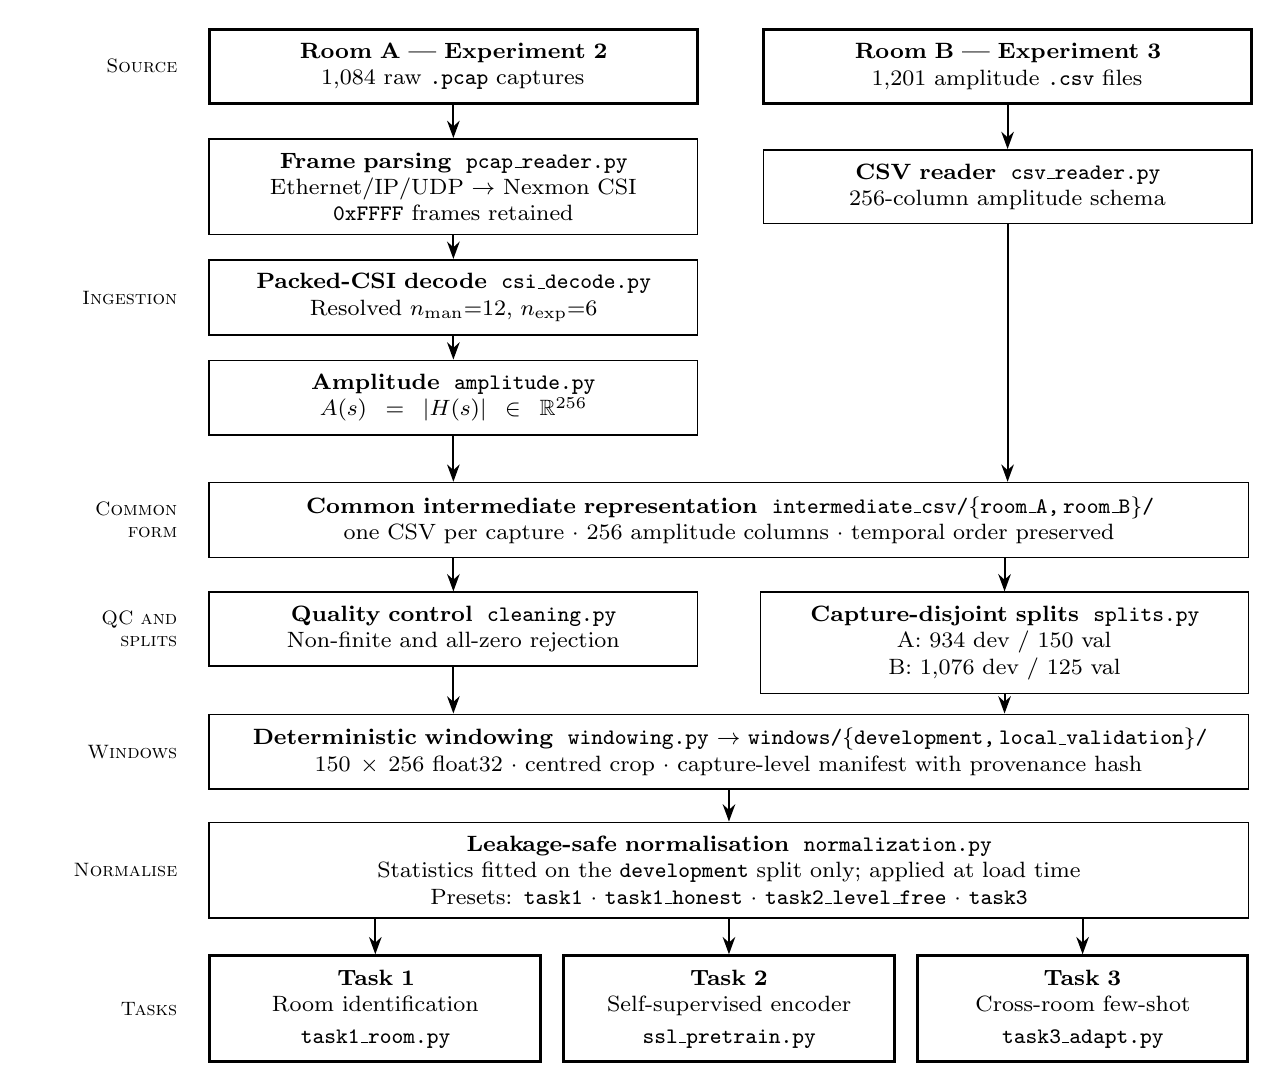
\begin{tikzpicture}[
  every node/.style={draw=black, fill=white, align=center, inner sep=5pt},
  box/.style   ={line width=0.6pt, minimum width=6.2cm, text width=5.6cm, font=\footnotesize},
  emph/.style  ={box, line width=1.1pt},
  wide/.style  ={box, line width=0.6pt, minimum width=13.2cm, text width=12.6cm},
  task/.style  ={box, line width=1.1pt, minimum width=4.2cm, text width=3.7cm},
  stage/.style ={draw=none, fill=none, font=\scriptsize\scshape, anchor=east, text width=1.9cm,
                 align=right, inner sep=0pt, xshift=-0.38cm},
  arr/.style   ={draw=black, line width=0.7pt, -{Stealth[length=2.2mm,width=1.6mm]}}
]

% ---------- sources ----------
\node[emph] (rawA) at (0,0)
  {\textbf{Room A \textemdash{} Experiment 2}\\1{,}084 raw \texttt{.pcap} captures};
\node[emph, right=0.8cm of rawA] (rawB)
  {\textbf{Room B \textemdash{} Experiment 3}\\1{,}201 amplitude \texttt{.csv} files};

% ---------- ingestion ----------
\node[box, below=0.42cm of rawA] (parse)
  {\textbf{Frame parsing}\; \texttt{pcap\_reader.py}\\
   Ethernet/IP/UDP $\to$ Nexmon CSI\\
   \texttt{0xFFFF} frames retained};
\node[box, below=0.30cm of parse] (decode)
  {\textbf{Packed-CSI decode}\; \texttt{csi\_decode.py}\\
   Resolved $n_{\mathrm{man}}{=}12$, $n_{\mathrm{exp}}{=}6$};
\node[box, below=0.30cm of decode] (ampA)
  {\textbf{Amplitude}\; \texttt{amplitude.py}\\
   $A(s)=|H(s)| \in \mathbb{R}^{256}$};
\node[box] (csvB) at (rawB |- parse)
  {\textbf{CSV reader}\; \texttt{csv\_reader.py}\\
   256-column amplitude schema};

% ---------- common form ----------
\node[wide, anchor=north] (inter) at ($(ampA.south)+(3.5,-0.58)$)
  {\textbf{Common intermediate representation}\; \texttt{intermediate\_csv/\{room\_A,\,room\_B\}/}\\
   one CSV per capture $\cdot$ 256 amplitude columns $\cdot$ temporal order preserved};

% ---------- QC and splits ----------
\node[box, below=0.42cm of inter.south west, anchor=north west] (clean)
  {\textbf{Quality control}\; \texttt{cleaning.py}\\
   Non-finite and all-zero rejection};
\node[box, below=0.42cm of inter.south east, anchor=north east] (splits)
  {\textbf{Capture-disjoint splits}\; \texttt{splits.py}\\
   A: 934 dev / 150 val \quad B: 1{,}076 dev / 125 val};

% ---------- windowing ----------
\node[wide, anchor=north] (windows) at ($(clean.south)!0.5!(splits.south)+(0,-0.42)$)
  {\textbf{Deterministic windowing}\; \texttt{windowing.py} $\to$ \texttt{windows/\{development,\,local\_validation\}/}\\
   $150 \times 256$ float32 $\cdot$ centred crop $\cdot$ capture-level manifest with provenance hash};

% ---------- normalisation ----------
\node[wide, below=0.40cm of windows] (norm)
  {\textbf{Leakage-safe normalisation}\; \texttt{normalization.py}\\
   Statistics fitted on the \texttt{development} split only; applied at load time\\
   Presets: \texttt{task1} $\cdot$ \texttt{task1\_honest} $\cdot$ \texttt{task2\_level\_free} $\cdot$ \texttt{task3}};

% ---------- tasks ----------
\node[task, below=0.45cm of norm.south west, anchor=north west] (t1)
  {\textbf{Task 1}\\Room identification\\[2pt]\texttt{task1\_room.py}};
\node[task, below=0.45cm of norm.south, anchor=north] (t2)
  {\textbf{Task 2}\\Self-supervised encoder\\[2pt]\texttt{ssl\_pretrain.py}};
\node[task, below=0.45cm of norm.south east, anchor=north east] (t3)
  {\textbf{Task 3}\\Cross-room few-shot\\[2pt]\texttt{task3\_adapt.py}};

% ---------- stage labels ----------
\node[stage] at (rawA.west  |- rawA)  {Source};
\node[stage] at (rawA.west  |- decode){Ingestion};
\node[stage] at (rawA.west  |- inter) {Common\\form};
\node[stage] at (rawA.west  |- clean) {QC and\\splits};
\node[stage] at (rawA.west  |- windows){Windows};
\node[stage] at (rawA.west  |- norm)  {Normalise};
\node[stage] at (rawA.west  |- t1)    {Tasks};

% ---------- arrows ----------
\draw[arr] (rawA)   -- (parse);
\draw[arr] (parse)  -- (decode);
\draw[arr] (decode) -- (ampA);
\draw[arr] (rawB)   -- (csvB);
\draw[arr] (ampA.south)   -- (ampA.south   |- inter.north);
\draw[arr] (csvB.south)   -- (csvB.south   |- inter.north);
\draw[arr] (clean.north   |- inter.south)   -- (clean.north);
\draw[arr] (splits.north  |- inter.south)   -- (splits.north);
\draw[arr] (clean.south)  -- (clean.south  |- windows.north);
\draw[arr] (splits.south) -- (splits.south |- windows.north);
\draw[arr] (windows) -- (norm);
\draw[arr] (norm.south -| t1) -- (t1.north);
\draw[arr] (norm.south -| t2) -- (t2.north);
\draw[arr] (norm.south -| t3) -- (t3.north);

\end{tikzpicture}
\caption{\textbf{End-to-end Python sensing, representation-learning and adaptation pipeline.}
  The two source archives are asymmetric: Room~A arrives as raw Nexmon \texttt{.pcap} and must be
  decoded to amplitude in Python, while Room~B is already amplitude \texttt{.csv}. Both are brought
  into one 256-column intermediate form, after which the pipeline is source-agnostic. The original
  capture is the atomic unit of the development/validation split, so every window derived from a
  capture stays on one side of it. Windows are stored un-normalised and a preset is applied at load
  time, which lets all three tasks share a single \texttt{windows/} directory. Both rooms use the
  same radio platform throughout: 5\,GHz, 80\,MHz, BCM4366c0 with Nexmon CSI extraction.}
\label{fig:pipeline_diagram}
\end{figure*}

\subsection{Empirical Bitfield Resolution for BCM4366c0 Packed CSI}
Experiment~2 archives provide raw ethernet PCAP captures extracted via Nexmon firmware~\cite{gringoli2019free} on a Broadcom BCM4366c0 transceiver operating at 80 MHz channel bandwidth. Each OFDM frame contains a 1024-byte CSI payload encoding 256 subcarriers as packed 32-bit words. A single word packs an in-phase mantissa ($I$), a quadrature mantissa ($Q$), and an exponent ($E$):
\begin{equation}
    W_{\text{packed}} = \left[ I \;\; (n_{\text{man}}\text{ bits}) \;\;|\;\; Q \;\; (n_{\text{man}}\text{ bits}) \;\;|\;\; E \;\; (n_{\text{exp}}\text{ bits}) \right]
\end{equation}
Rather than transcribing parameters from external sources, we resolved the exact bitfield configuration empirically by formulating a physical null-subcarrier alignment objective (\texttt{src/csi\_decode.py --resolve}). Under IEEE 802.11ac VHT80 standards, fixed subcarrier positions are reserved as guard bands ($\pm 128 \dots \pm 123$), DC pilot carriers (center 3 bins), and null notches, where transmitted RF power is zero. Because Room~B data was provided as pre-computed amplitude CSVs from the identical platform, physical null locations in Room~A must strictly align with Room~B.

We evaluated all structurally valid candidate layouts $(n_{\text{man}}, n_{\text{exp}})$ satisfying $2n_{\text{man}} + n_{\text{exp}} \le 32$. Bit occupancy analysis across $2,010,000$ packed words revealed that bits 30--31 are perpetually zero, while bit 5 is constantly 1 (denoting a negative sign in two's-complement exponent space). Evaluating the ratio of null-subcarrier amplitude to data-subcarrier median across layouts revealed that candidate $(12, 6)$ with exponent application uniquely produces a ratio of $\mathbf{0.020}$, perfectly matching Room~B's physical null ratio of $\mathbf{0.024}$ (the overlaid null-alignment plot is \texttt{figures/decode\_validation.png} in the repository). Omitting the exponent yields an invalid ratio of $0.78$--$1.01$, obliterating the 802.11ac channel notch structure. The real and imaginary components are sign-extended as 12-bit two's complement integers:
\begin{equation}
    H(s) = \left( \text{SignExt}_{12}(I) + j \cdot \text{SignExt}_{12}(Q) \right) \cdot 2^{\text{SignExt}_6(E)}
\end{equation}
The amplitude is extracted as $A(s) = |H(s)| = \sqrt{I_{\text{scaled}}^2 + Q_{\text{scaled}}^2} \in \mathbb{R}$.


\subsection{Discovery of the Nexmon Frame-Interleaving Hardware Artifact}
Inspecting the Experiment~2 PCAPs revealed an undocumented transmission artifact: in every Room~A capture, frames alternate between standard 802.11 frames with incrementing sequence numbers and secondary frames whose sequence-control field reads \texttt{0xFFFF}, arriving $\sim$0.4~ms later. These are not corrupt --- $976$--$992$ of their $1024$ payload bytes are non-zero and their amplitude distribution matches the sequenced frames --- and discarding them cuts the median observation count per capture from $221$ to $\mathbf{111}$, putting \textbf{all 1,084 Room~A captures} below the official $T_{\text{win}}=150$. Both streams must therefore be retained.

However, retaining the interleaved frames introduces a profound temporal distortion: consecutive observations bounce between two distinct transmitter states, introducing strong negative lag-1 autocorrelation ($r_1 \in [-0.15, -0.66]$, mean $-0.327 \pm 0.165$). In contrast, Room~B exhibits smooth, near-zero lag-1 autocorrelation ($r_1 = +0.035 \pm 0.072$). As established in Section~\ref{sec:task1} and Section~\ref{sec:task2}, this hardware artifact acts as a powerful spurious shortcut for machine learning models.

\subsection{Data Cleaning, Quality Control \& Windowing}
\textbf{Quality Control (\texttt{src/cleaning.py}):} We instituted automated filters to reject corrupt data: (i)~captures with non-finite or NaN values, (ii)~frames with all-zero subcarriers ($A(s) = 0, \forall s$), and (iii)~duplicate captures. In the course archive, file \texttt{stand65(1).pcap} was identified as a byte-identical copy of \texttt{stand65.pcap}; it was quarantined to prevent index drift.

\noindent\textbf{Deterministic Centered Windowing (\texttt{src/windowing.py}):} Raw Room~A captures vary between $112$ and $251$ observations (median $221$), while Room~B captures contain exactly $500$ rows. For each capture, a deterministic centered window of length $T_{\text{win}}=150$ is extracted without inspecting labels:
\begin{equation}
    t_{\text{start}} = \max\left(0, \frac{N_{\text{obs}} - 150}{2}\right), \quad t_{\text{end}} = t_{\text{start}} + 150
\end{equation}
Twelve Room~A captures contained fewer than $150$ observations (including three captures in the official validation set). To preserve the exact challenge validation denominator, short captures were reflect-padded at boundary frames and cataloged via the boolean flag \texttt{was\_padded} in \texttt{windows/manifest.csv}. Every generated window is stamped with a SHA-256 provenance hash (\texttt{2a323eeb9765}) tying it to \texttt{configs/experiment.yaml}.

\subsection{Leakage-Safe Normalization Framework}
To strictly enforce Section~8 leakage controls, normalization statistics are fitted exclusively on development captures ($split == \text{development}$) via \texttt{src/normalization.py}. Windows are saved to disk in un-normalized float32 format, allowing downstream models to evaluate distinct normalization presets at load time without data re-ingestion:
\texttt{task1} (global scope) preserves absolute amplitude across rooms; \texttt{task1\_subband} additionally centres each 20\,MHz sub-band, neutralising the $4\times$ AGC step at subcarriers 137--187; \texttt{task1\_honest} (per-window scope) standardises every window to $\mu=0,\sigma=1$, stripping all static multipath and gain signatures. \texttt{task2} and \texttt{task2\_level\_free} are two-channel: channel~0 carries $\ln(1+A_{t,s})$ after scaling and channel~1 subtracts the per-subcarrier temporal mean, isolating dynamics; \texttt{task2\_level\_free} divides each window by a single scalar, removing absolute energy while preserving spectral shape. \texttt{task3} standardises features with room-specific development statistics (AdaBN).

% =========================================================================
\section{Evaluation Protocol \& Leakage Controls}
% =========================================================================

\subsection{Capture-Level Isolation \& Partition Integrity}
The atomic unit of partitioning is the original capture. Multiple temporal slices from the same physical capture are strictly prohibited from bridging the development and validation split. All leakage constraints mandated by Section~8 and Section~9 were programmatically verified through automated unit tests (\texttt{tests/test\_no\_leakage.py}):
\begin{enumerate}
    \item \textbf{Room A:} the supplied \texttt{validation/} directory, 25 captures per activity ($25\times6=150$); the remaining 934 are development.
    \item \textbf{Room B:} no validation directory is supplied, so we sorted all candidate filenames deterministically and drew 25 per class with the public seed \textbf{42} ($25\times5=125$), leaving 1,076 development captures. The exact partition is serialised to \texttt{results/room\_B\_validation\_seed42.json} for audit.
    \item \textbf{Validation isolation:} validation captures are never used for model fitting, pretraining, feature selection or hyperparameter search.
    \item \textbf{Metadata ban:} filenames, extensions, observation counts and timestamps are stripped from model inputs.
\end{enumerate}
Table~\ref{tab:dataset_composition} reports the final capture and window counts across all splits.

\begin{table}[htbp]
\centering
\footnotesize
\setlength{\tabcolsep}{4pt}
\caption{Capture-Disjoint Dataset Partitioning Across Rooms and Splits.}
\label{tab:dataset_composition}
\begin{tabular}{lrr@{\hspace{2.2em}}lrr}
\toprule
\multicolumn{3}{c}{\textbf{Room A (Experiment 2)}} & \multicolumn{3}{c}{\textbf{Room B (Experiment 3)}} \\
\cmidrule(lr){1-3} \cmidrule(lr){4-6}
\textbf{Activity} & \textbf{Dev} & \textbf{Val} & \textbf{Activity} & \textbf{Dev} & \textbf{Val} \\
\midrule
\textsc{Fall}      & 177 & 25 & \textsc{Empty}  & 242 & 25 \\
\textsc{Sit}       & 178 & 25 & \textsc{Lying}  & 326 & 25 \\
\textsc{Sit-Down}  & 155 & 25 & \textsc{Sit}    & 128 & 25 \\
\textsc{Stand}     & 115 & 25 & \textsc{Stand}  & 196 & 25 \\
\textsc{Stand-Up}  & 155 & 25 & \textsc{Walk}   & 184 & 25 \\
\textsc{Walk}      & 154 & 25 & ---             & --- & --- \\
\midrule
\textbf{Total} & \textbf{934} & \textbf{150} & \textbf{Total} & \textbf{1,076} & \textbf{125} \\
\bottomrule
\end{tabular}
\end{table}

% =========================================================================
\section{Task 1: Recorded-Environment Identification}
\label{sec:task1}
% =========================================================================

\subsection{The Illusion of Universal Room Fingerprinting}
Task~1 asks whether a $150 \times 256$ window came from Room~A or Room~B. On globally normalised features a logistic regression reaches a perfect $\mathbf{1.0000}$ ($275/275$). Reporting that as an environment fingerprint would be wrong: Figure~\ref{fig:task1_window_length} shows the same $\mathbf{1.0000}$ at $T_{\text{win}}=1$, and a single observation carries no temporal multipath information. The classifier is reading an arbitrary $\sim$$\mathbf{490\times}$ amplitude gap between our Python-decoded Room~A values and the integer scaling of Room~B's supplied CSVs.

\begin{figure}[htbp]
\centering
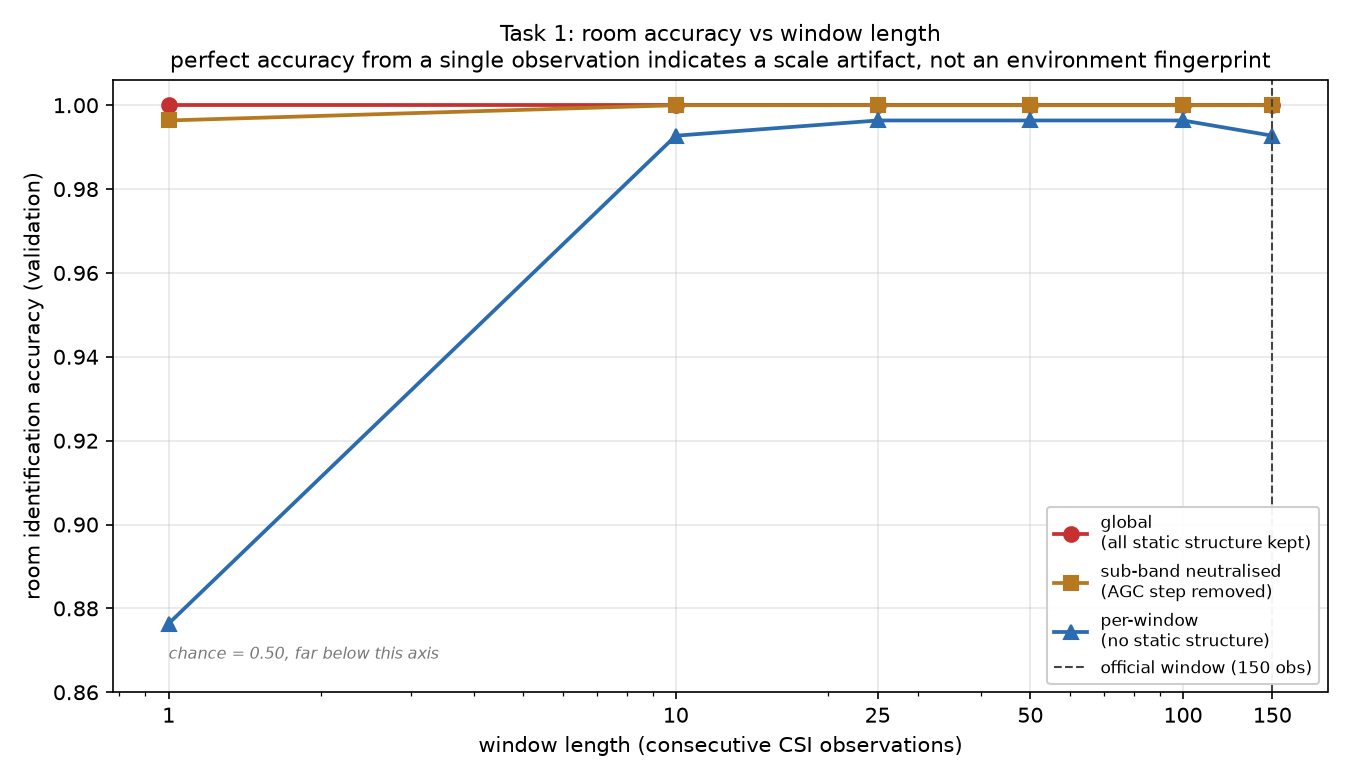
\includegraphics[width=0.44\linewidth]{figures/task1_accuracy_vs_window_length.png}
\caption{Task 1: Environment classification accuracy vs window length $T_{\text{win}} \in \{1, 10, 25, 50, 100, 150\}$. Naive presets achieve 1.000 accuracy at $T=1$ due to the global scale artifact.}
\label{fig:task1_window_length}
\end{figure}

\subsection{Systematic Ablation Ladder}
To isolate the true sources of discriminability, we constructed a progressive ablation ladder (\texttt{src/task1\_ablation.py}). We evaluated models across four feature rungs, selectively disabling static and dynamic channel dimensions:
Each rung removes one further source of discriminability (Table~\ref{tab:task1_results}). \texttt{task1} keeps the raw scale. \texttt{task1\_subband} subtracts sub-band medians, neutralising Room~A's $4\times$ AGC step at subcarriers 137--187; accuracy is unchanged, so the scale discrepancy is present uniformly across all 256 bins rather than confined to that band. \texttt{task1\_honest} standardises each window to $\mu=0,\sigma=1$, erasing every static multipath profile, global scale difference and sub-band offset, yet accuracy falls only to $0.9927$ ($273/275$). Finally, restricting Room~A ingestion to sequenced frames removes the Nexmon interleaving artifact and drops accuracy to $0.9418$ --- the largest single drop in the ladder, and evidence that \texttt{task1\_honest} was keying on interleaving rather than on the environment.


\begin{table}[htbp]
\centering
\footnotesize
\setlength{\tabcolsep}{4pt}
\caption{Task 1 Ablation Ladder: Unmasking the Session Confound.}
\label{tab:task1_results}
\begin{tabular}{llcc}
\toprule
\textbf{Ablation Rung} & \textbf{Information Removed} & \textbf{Accuracy ($T=150$)} & \textbf{Accuracy ($T=1$)} \\
\midrule
\texttt{task1} (Global) & None ($\sim$490$\times$ scale preserved) & 1.0000 & 1.0000 \\
\texttt{task1\_subband} & Sub-band AGC step removed & 1.0000 & 0.9964 \\
\texttt{task1\_honest} & Static profile \& scale removed & 0.9927 & 0.8764 \\
\texttt{task1\_honest} (Sequenced only) & Frame interleaving removed & 0.9418 & --- \\
\bottomrule
\end{tabular}
\end{table}

\subsection{Finding: Confounding of Room and Session Dynamics}
Table~\ref{tab:task1_results} shows environment recognition here is confounded by recording session and acquisition artifacts (specification Section~12.1). Even at the strictest rung, Room~A runs at an effective $\sim$30~Hz with clock jitter while Room~B is a uniform 500-sample sequence, so the environment stays identifiable without any architectural feature being learned. Task~1 is therefore a serviceable router for Task~3, but not a claim of generalised physical room sensing.

% =========================================================================
\section{Task 2: Self-Supervised CSI Representation Learning}
\label{sec:task2}
% =========================================================================

\subsection{Self-Supervised Architecture \& Pretraining Objective}
Task~2 requires learning a generalized feature encoder on the 2,010 development windows from both rooms without using activity or room labels. Given the limited dataset scale, large Transformer backbones severely overfit. We designed a compact 1D Dilated Residual Convolutional Neural Network (\texttt{src/encoder.py}) comprising 280,000 parameters:
The input $X \in \mathbb{R}^{150 \times 256 \times 2}$ is flattened along channels to 512 features per time step; a $1\times1$ convolution projects these to 64 maps; three residual blocks of kernel size 5 and dilations $d \in \{1,2,4\}$ with 128 channels widen the receptive field across the window; concatenated mean and max temporal pooling gives 256 dimensions, projected linearly to an embedding $z \in \mathbb{R}^{128}$.

\noindent\textbf{Contrastive Objective (SimCLR~\cite{chen2020simple}):} The encoder was pretrained using the Normalized Temperature-scaled Cross-Entropy (NT-Xent) loss with temperature $\tau = 0.2$ and batch size 128 for 200 epochs using AdamW ($\eta = 10^{-3}$, weight decay $10^{-4}$) with cosine learning rate decay:
\begin{equation}
    \mathcal{L}_{\text{NT-Xent}} = -\log \frac{\exp(\text{sim}(z_i, z_j) / \tau)}{\sum_{k=1}^{2B} \mathbb{I}_{[k \ne i]} \exp(\text{sim}(z_i, z_k) / \tau)}
\end{equation}
Pretraining was conducted strictly on development data; no validation samples, early stopping, or checkpoint selections were permitted.

\subsection{Adjacency-Breaking Augmentations for Frame Interleaving}
Because Room~A alternates between two frame streams ($r_1 = -0.33$), naive contrastive learning creates an undesirable shortcut: the encoder minimizes loss simply by identifying the frame-interleaving signature, failing to learn somatic kinematics. To force the network to learn invariant motion dynamics, we introduced two specialized augmentations alongside standard transforms:
\begin{enumerate}
    \item \textbf{Stride-2 Subsampling with Random Phase:} Subsamples alternating frames ($t \in \{0, 2, \dots\}$ or $t \in \{1, 3, \dots\}$), isolating a single frame stream and removing the alternation artifact.
    \item \textbf{Local Temporal Shuffling:} Shuffles observations within local 4-sample blocks, breaking strict lag-1 phase coherence.
    \item \textbf{Standard Augmentations:} Random temporal cropping ($60\%$--$100\%$ resized to 150 steps), contiguous subcarrier masking (up to 32 bins), per-subcarrier gain perturbation, additive Gaussian noise ($\sigma = 0.05$), and temporal reversal.
\end{enumerate}

\subsection{Baselines \& Linear-Probe Evaluation Protocol}
To benchmark the learned representation, we froze the encoder weights and trained a multinomial logistic regression probe with balanced class weights on labeled development data, scoring performance on the fixed 275-sample validation set. The probe's regularization parameter $C$ was selected from $\{10^{-3}, \dots, 10^{2}\}$ using capture-grouped 5-fold cross-validation on development data. Two baselines are mandatory. The \textbf{domain-engineered kinematic features} (416 dimensions) split the subcarriers into 16 spectral groups and take ten statistics per group --- mean, standard deviation, dynamic range, skewness, kurtosis, mean absolute first difference, and spectral energy in four temporal bands ($[0,0.5)$, $[0.5,1.5)$, $[1.5,3.0)$, $[3.0,6.0)$\,Hz) --- concatenated with the temporal variance of all 256 subcarriers. The \textbf{random-weight} baseline is the identical architecture with frozen Gaussian weights, its BatchNorm running statistics re-estimated on development data without labels.

\begin{table}[htbp]
\centering
\footnotesize
\setlength{\tabcolsep}{4pt}
\caption{Task 2 Linear-Probe Benchmark: 8-Class Validation Performance (Mean $\pm$ Std across 3 pretraining seeds).}
\label{tab:task2_results}
\begin{tabular}{lcccc}
\toprule
\textbf{Representation} & \textbf{Overall Macro-F1} & \textbf{Balanced Acc.} & \textbf{Room A F1} & \textbf{Room B F1} \\
\midrule
Handcrafted Kinematic Features (416-d) & 0.893 & 0.895 & 0.872 & 0.912 \\
Random-Weight Architecture & 0.616 $\pm$ 0.008 & 0.637 $\pm$ 0.006 & 0.517 $\pm$ 0.011 & 0.712 $\pm$ 0.021 \\
\textbf{SimCLR SSL (All Augmentations)} & \textbf{0.924 $\pm$ 0.013} & \textbf{0.928 $\pm$ 0.014} & \textbf{0.912 $\pm$ 0.012} & 0.950 $\pm$ 0.016 \\
SimCLR SSL (No Adjacency Break) & 0.901 $\pm$ 0.020 & 0.902 $\pm$ 0.019 & 0.869 $\pm$ 0.042 & \textbf{0.951 $\pm$ 0.010} \\
\bottomrule
\end{tabular}
\end{table}



\subsection{Experimental Findings \& Representation Analysis}
Table~\ref{tab:task2_results} presents the quantitative results:
\begin{enumerate}
    \item \textbf{Pretraining Efficacy:} Contrastive pretraining lifts the identical architecture from $0.616$ (random weights) to $\mathbf{0.924}$ Macro-F1, a gain of $30.8$ points. The learned representation also \emph{exceeds} the 416-dimensional handcrafted kinematic baseline ($0.893$) by $3.1$ points overall, by $4.0$ points in Room~A ($0.912$ vs $0.872$) and by $3.8$ points in Room~B ($0.950$ vs $0.912$). Self-supervision on unlabelled CSI therefore recovers more activity-relevant structure than hand-designed spectral features.
    \item \textbf{Ablation of Adjacency-Breaking Augmentations:} Omitting stride-2 subsampling and local shuffling costs $2.3$ points of Macro-F1 ($0.924 \to 0.901$). The entire loss falls on Room~A ($0.912 \to 0.869$), the only room exhibiting frame interleaving; Room~B is unaffected ($0.950 \to 0.951$). Critically, the ablated variant converges to a \emph{lower} contrastive loss ($1.406 \pm 0.007$ vs $1.689 \pm 0.006$): retaining the frame alternation lets the encoder match positive pairs trivially, so the pretext objective becomes easier to minimise while the resulting representation is measurably worse. A lower SimCLR loss is thus not evidence of a better encoder, and breaking temporal adjacency is necessary to prevent the shortcut.
    \item \textbf{Qualitative UMAP Diagnosis:} Figure~\ref{fig:task2_umap} displays 2-D UMAP projections of frozen embeddings. The representation splits completely by room ($100\%$ linear separation). Within each room, semantically active classes form distinct, coherent clusters, while static postures (\textsc{Sit} vs \textsc{Stand}) exhibit slight overlap.
    \item \textbf{Zero-Shot Cross-Room Activity Failure:} In a development-only diagnostic, training a probe on \textsc{Sit}, \textsc{Stand}, \textsc{Walk} in one room and evaluating on the other yielded Macro-F1 between $\mathbf{0.015}$ and $\mathbf{0.382}$ against a three-class chance level of $0.167$. Without per-room standardisation every configuration sits at or below chance ($0.083$--$0.186$). Standardisation helps only asymmetrically: it lifts the SSL representation into Room~A to $\mathbf{0.382}$, but leaves Room~B at $0.185$ and drives the handcrafted features into Room~B down to $0.015$. No configuration transfers shared activities reliably in both directions, indicating that the learned representations do not align identical activities across disparate rooms.
\end{enumerate}

\begin{figure}[htbp]
\centering
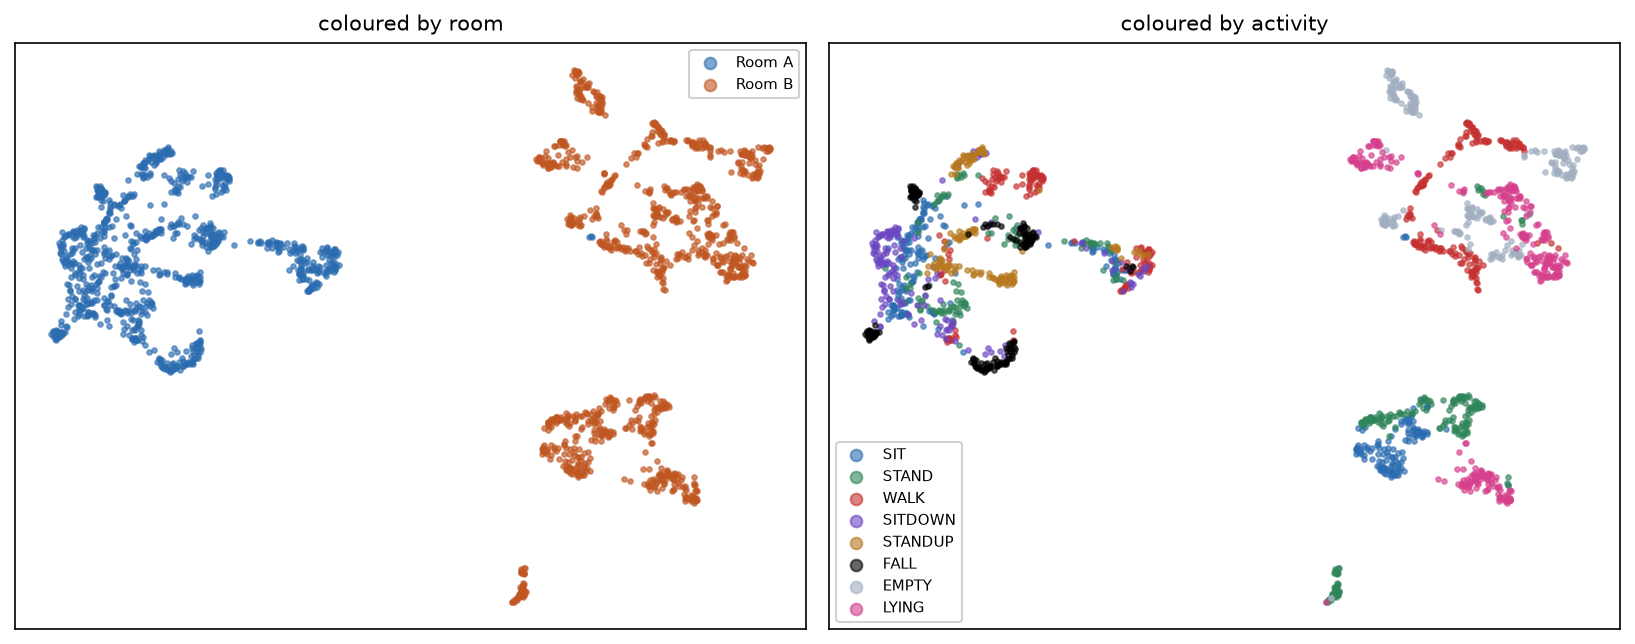
\includegraphics[width=0.70\linewidth]{figures/task2_umap_ssl.png}
\caption{Task 2 encoder diagnosis: 2-D UMAP of the frozen SimCLR embeddings, coloured by room (left) and by activity (right). The representation separates the two rooms completely; within each room dynamic activities form coherent clusters, while \textsc{Sit} and \textsc{Stand} overlap. The equivalent projections for the handcrafted, random-weight and no-adjacency-break representations are in \texttt{figures/task2\_umap.png} in the repository.}
\label{fig:task2_umap}
\end{figure}

% =========================================================================
\section{Task 3: Cross-Room Few-Label Adaptation}
\label{sec:task3}
% =========================================================================

\subsection{Few-Shot Adaptation Architecture}
We evaluate both transfer directions under the protocol set out in Section~1.3.

\noindent\textbf{Prototypical Alignment~\cite{snell2017prototypical}:} Using frozen embeddings $z \in \mathbb{R}^{128}$ from the Task~2 encoder, we apply per-room standardization (\texttt{task3} preset) to align source and target feature distributions (AdaBN). For each activity $c$, class prototypes $\mu_c$ are computed as:
\begin{align}
    \mu_c^{\text{shared}} &= \frac{1}{|D_{\text{src}, c}|} \sum_{x \in D_{\text{src}, c}} z(x) \quad (c \in \mathcal{Y}_{\text{shared}}) \\
    \mu_c^{\text{exclusive}} &= \frac{1}{K} \sum_{x \in S_{\text{tgt}, c}} z(x) \quad (c \in \mathcal{Y}_{\text{tgt} \setminus \text{src}})
\end{align}
Inference assigns validation query $x$ to the nearest prototype via cosine similarity:
\begin{equation}
    \hat{y} = \arg\max_{c \in \mathcal{Y}_{\text{tgt}}} \frac{z(x) \cdot \mu_c}{\|z(x)\| \|\mu_c\|}
\end{equation}

\noindent\textbf{Semi-Supervised Refinement (\texttt{refined}):} We implemented an iterative soft $k$-means expectation-maximization over unlabeled target development captures. Initialized at the base prototypes, cluster assignments are iteratively updated while anchoring target-exclusive prototypes to their $K$ support captures.

\noindent\textbf{Support Sampling Protocol:} Support sets were sampled strictly at the capture level from target development data across 10 deterministic random seeds. For each $K$, evaluations were repeated across 3 encoder pretraining seeds ($10 \times 3 = 30$ runs per configuration).

\subsection{The Level-Free Rerun \& Retraction of Spurious Transfer}
Under the original global \texttt{task2} preset, handcrafted features with soft $k$-means refinement appeared to transfer shared activities into Room~B at a shared Macro-F1 of $\mathbf{0.236}$. Auditing showed this was a data artifact. Room~B \textsc{Walk} captures are the only files in the archive lacking the \texttt{\_Amp\_} filename substring, and their mean amplitude is $\mathbf{50\%}$ above every other Room~B class ($473$ vs $304$--$358$); a scalar amplitude threshold alone separates \textsc{Walk} from the rest at \textbf{ROC-AUC 0.898}. Because \texttt{RoomScaler} standardises per room and this is a per-\emph{class} offset inside one room, it passed straight through into the prototypes.

The \texttt{task2\_level\_free} preset divides each window by its own scalar energy, removing absolute level while preserving spectral shape (\textsc{Walk} level AUC $0.894 \to 0.693$). After retraining every encoder and rerunning Task~3, the handcrafted shared F1 in Room~B collapsed from $0.236$ to $\mathbf{0.038}$. \textbf{We retract that transfer claim}: the earlier gain was entirely artifactual. All results reported here are from the level-free rerun.

\subsection{Quantitative Results \& Label Efficiency Curves}
Table~\ref{tab:task3_headline} presents the corrected headline validation results at $K=5$ under oracle routing. Figure~\ref{fig:task3_efficiency} illustrates the label-efficiency progression as $K$ increases from 1 to 20.

\begin{table}[htbp]
\centering
\footnotesize
\setlength{\tabcolsep}{4pt}
\caption{Task 3 Few-Shot Adaptation Benchmark at $K=5$ (Oracle Routing, Validation Set, 30 Runs).}
\label{tab:task3_headline}
\begin{tabular}{llcccccc}
\toprule
& & \multicolumn{3}{c}{\textbf{Target Room A} ($\mathcal{B} \to \mathcal{A}$)} & \multicolumn{3}{c}{\textbf{Target Room B} ($\mathcal{A} \to \mathcal{B}$)} \\
\cmidrule(lr){3-5} \cmidrule(lr){6-8}
\textbf{Features} & \textbf{Method} & \textbf{Overall F1} & \textbf{Exclusive F1} & \textbf{Shared F1} & \textbf{Overall F1} & \textbf{Exclusive F1} & \textbf{Shared F1} \\
\midrule
\textbf{SSL Full} & Prototype & $0.240 \pm 0.043$ & $\mathbf{0.390 \pm 0.075}$ & $0.090 \pm 0.042$ & $\mathbf{0.337 \pm 0.068}$ & $\mathbf{0.525 \pm 0.077}$ & $0.211 \pm 0.082$ \\
SSL Full & Refined & $0.241 \pm 0.055$ & $0.308 \pm 0.076$ & $0.173 \pm 0.084$ & $0.295 \pm 0.092$ & $0.466 \pm 0.109$ & $0.181 \pm 0.127$ \\
Handcrafted & Prototype & $\mathbf{0.268 \pm 0.041}$ & $0.448 \pm 0.077$ & $0.089 \pm 0.017$ & $0.170 \pm 0.032$ & $0.411 \pm 0.072$ & $0.009 \pm 0.011$ \\
Handcrafted & Refined & $0.232 \pm 0.014$ & $0.330 \pm 0.033$ & $0.134 \pm 0.021$ & $0.160 \pm 0.017$ & $0.343 \pm 0.037$ & $0.038 \pm 0.025$ \\
\midrule
\multicolumn{2}{l}{\textit{Uniform Random Guessing}} & \multicolumn{3}{c}{$\approx 0.167$ (6 classes)} & \multicolumn{3}{c}{$\approx 0.200$ (5 classes)} \\
\bottomrule
\end{tabular}
\end{table}

\begin{figure}[htbp]
\centering
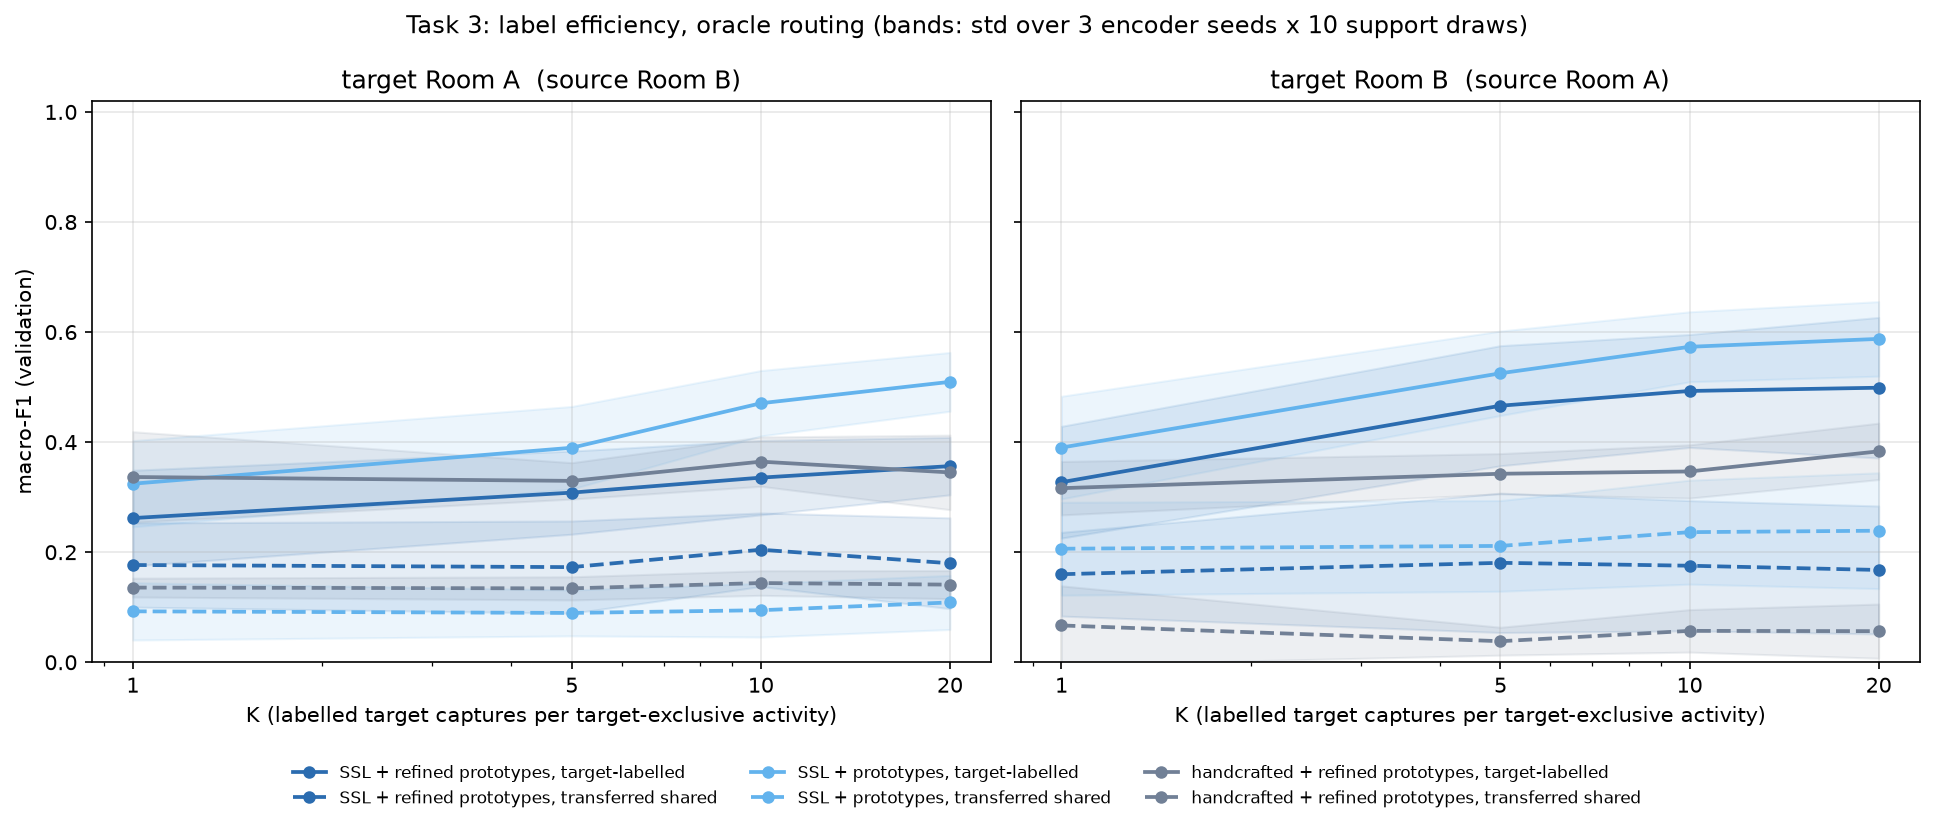
\includegraphics[width=0.44\linewidth]{figures/task3_label_efficiency.png}
\caption{Task 3 label efficiency curves: Macro-F1 vs $K \in \{1, 5, 10, 20\}$ for Target Room~A and Room~B, showing scaling on target-exclusive classes vs stagnation on shared classes.}
\label{fig:task3_efficiency}
\end{figure}

\begin{enumerate}
    \item \textbf{Target-exclusive activities scale with $K$:} Room~A rises from $0.324 \pm 0.078$ at $K=1$ to $\mathbf{0.510 \pm 0.053}$ at $K=20$, Room~B from $0.390 \pm 0.093$ to $\mathbf{0.588 \pm 0.068}$. Few-shot prototypes do capture novel activities.
    \item \textbf{Shared transfer does not scale at all:} it sits near chance throughout ($0.090$ in Room~A against chance $0.167$; $0.211$ in Room~B against $0.200$), so source-room prototypes never align with target-room signals however many target-exclusive labels are added.
    \item \textbf{Unsupervised refinement hurts:} soft $k$-means lowers Room~B Macro-F1 ($0.337 \to 0.295$), because target embeddings cluster by session rather than activity and the updates drag prototypes off the true class centres.
\end{enumerate}

\subsection{Optimal Hungarian Diagnostic \& Confusion Matrix Analysis}
To determine whether shared transfer failed due to poor prototype calibration or fundamental kinematic confusion, we computed the optimal bipartite Hungarian matching between predicted clusters and true validation labels (\texttt{src/task3\_diagnostics.py}).

As shown in Table~\ref{tab:hungarian_bound}, even under an oracle permutation that optimally reassigns predicted classes to ground-truth labels, the upper bound on shared Macro-F1 reaches only $\mathbf{0.251}$ in Room~A and $\mathbf{0.305}$ in Room~B. In Room~B, the optimal assignment swaps \textsc{Sit} and \textsc{Walk} ($\textsc{Sit} \leftrightarrow \textsc{Walk}$). 

Inspection of the $K=5$ confusion matrix (Figure~\ref{fig:task3_confusion}) and the per-activity breakdown (Table~\ref{tab:task3_per_activity}) confirms this pathology: in Room~B, $\mathbf{49.1\%}$ of true \textsc{Sit} windows ($368/750$) and $\mathbf{37.5\%}$ of \textsc{Stand} windows ($281/750$) are misclassified as \textsc{Walk}, while $\mathbf{35.3\%}$ of \textsc{Walk} windows are classified as \textsc{Empty}. In Room~A, static postures collapse into dynamic transitions: $34.3\%$ of \textsc{Sit} windows are misclassified as \textsc{Sit-Down}, and $30.5\%$ are misclassified as \textsc{Fall}. Thus, failure to transfer is not an algorithmic defect of the classifier, but a consequence of environment-specific multipath altering the frequency and variance characteristics of human motion.

\begin{table}[htbp]
\centering
\footnotesize
\setlength{\tabcolsep}{4pt}
\caption{Hungarian optimal-assignment diagnostic: the best Macro-F1 reachable by any one-to-one relabelling of the predicted classes. The optimal permutation swaps \textsc{Sit}$\leftrightarrow$\textsc{Walk} in \emph{both} directions (Room~A additionally swaps \textsc{Stand}$\leftrightarrow$\textsc{Fall}); all other activities map to themselves. This is an \emph{oracle} computed from validation labels --- a diagnostic upper bound, never an achieved result.}
\label{tab:hungarian_bound}
\begin{tabular}{lcccc}
\toprule
\textbf{Target Room} & \textbf{Macro-F1} & \textbf{Bound} & \textbf{Shared F1} & \textbf{Bound} \\
\midrule
Room A ($\mathcal{B} \to \mathcal{A}$) & 0.243 & 0.255 & 0.177 & 0.251 \\
Room B ($\mathcal{A} \to \mathcal{B}$) & 0.292 & 0.366 & 0.182 & 0.305 \\
\bottomrule
\end{tabular}
\end{table}

\begin{figure}[htbp]
\centering
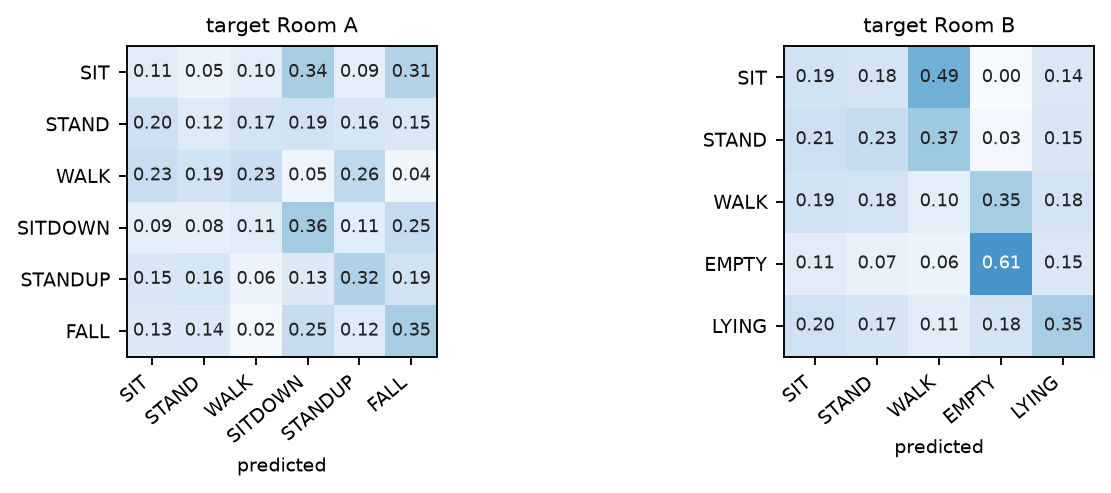
\includegraphics[width=0.82\linewidth]{figures/task3_confusion_K5_compact.png}
\caption{Task 3 row-normalised confusion at $K=5$; configuration as in Table~\ref{tab:task3_per_activity}. Room~B collapses \textsc{Sit} and \textsc{Stand} into \textsc{Walk}; Room~A collapses static postures into transitions.}
\label{fig:task3_confusion}
\end{figure}

\begin{table}[htbp]
\centering
\footnotesize
\setlength{\tabcolsep}{4pt}
\caption{Per-activity precision, recall and F1 at $K=5$ (specification Section~11): SSL encoder, refined prototypes, oracle routing, pooled over 30 runs ($3$ seeds $\times\,10$ draws, 750 windows per class). Every shared activity --- transferred with no target label --- scores below every target-exclusive activity learned from just $K=5$ captures.}
\label{tab:task3_per_activity}
\begin{tabular}{lrrr@{\hspace{1.6em}}lrrr}
\toprule
\multicolumn{4}{c}{\textbf{Target Room A} ($\mathcal{B} \to \mathcal{A}$)} & \multicolumn{4}{c}{\textbf{Target Room B} ($\mathcal{A} \to \mathcal{B}$)} \\
\cmidrule(lr){1-4} \cmidrule(lr){5-8}
\textbf{Activity} & \textbf{P} & \textbf{R} & \textbf{F1} & \textbf{Activity} & \textbf{P} & \textbf{R} & \textbf{F1} \\
\midrule
\multicolumn{8}{l}{\textit{Shared --- transferred from the source room, no target labels}} \\
\textsc{Sit}       & 0.121 & 0.111 & 0.116 & \textsc{Sit}    & 0.211 & 0.191 & 0.200 \\
\textsc{Stand}     & 0.166 & 0.124 & 0.142 & \textsc{Stand}  & 0.280 & 0.235 & 0.255 \\
\textsc{Walk}      & 0.337 & 0.229 & 0.273 & \textsc{Walk}   & 0.085 & 0.096 & 0.090 \\
\addlinespace[2pt]
\multicolumn{8}{l}{\textit{Target-exclusive --- learned from $K=5$ labelled captures}} \\
\textsc{Sit-Down}  & 0.272 & 0.357 & 0.309 & \textsc{Empty}  & 0.522 & 0.609 & 0.562 \\
\textsc{Stand-Up}  & 0.300 & 0.320 & 0.309 & \textsc{Lying}  & 0.360 & 0.348 & 0.354 \\
\textsc{Fall}      & 0.274 & 0.349 & 0.307 & ---             & ---   & ---   & --- \\
\midrule
\textbf{Macro-F1}  &       &       & \textbf{0.243} & \textbf{Macro-F1} & & & \textbf{0.292} \\
\bottomrule
\end{tabular}
\end{table}

\subsection{Routing Contribution Ablation}
We evaluated the contribution of environment-aware routing by comparing three operational configurations:
\emph{oracle} routing sends each window to its true room's prototype bank; \emph{predicted} routing uses the Task~1 classifier on the \texttt{task1\_honest} preset ($99.27\%$ accuracy); \emph{no} routing evaluates a single global bank over all eight activities without environment conditioning.

\begin{figure}[htbp]
\centering
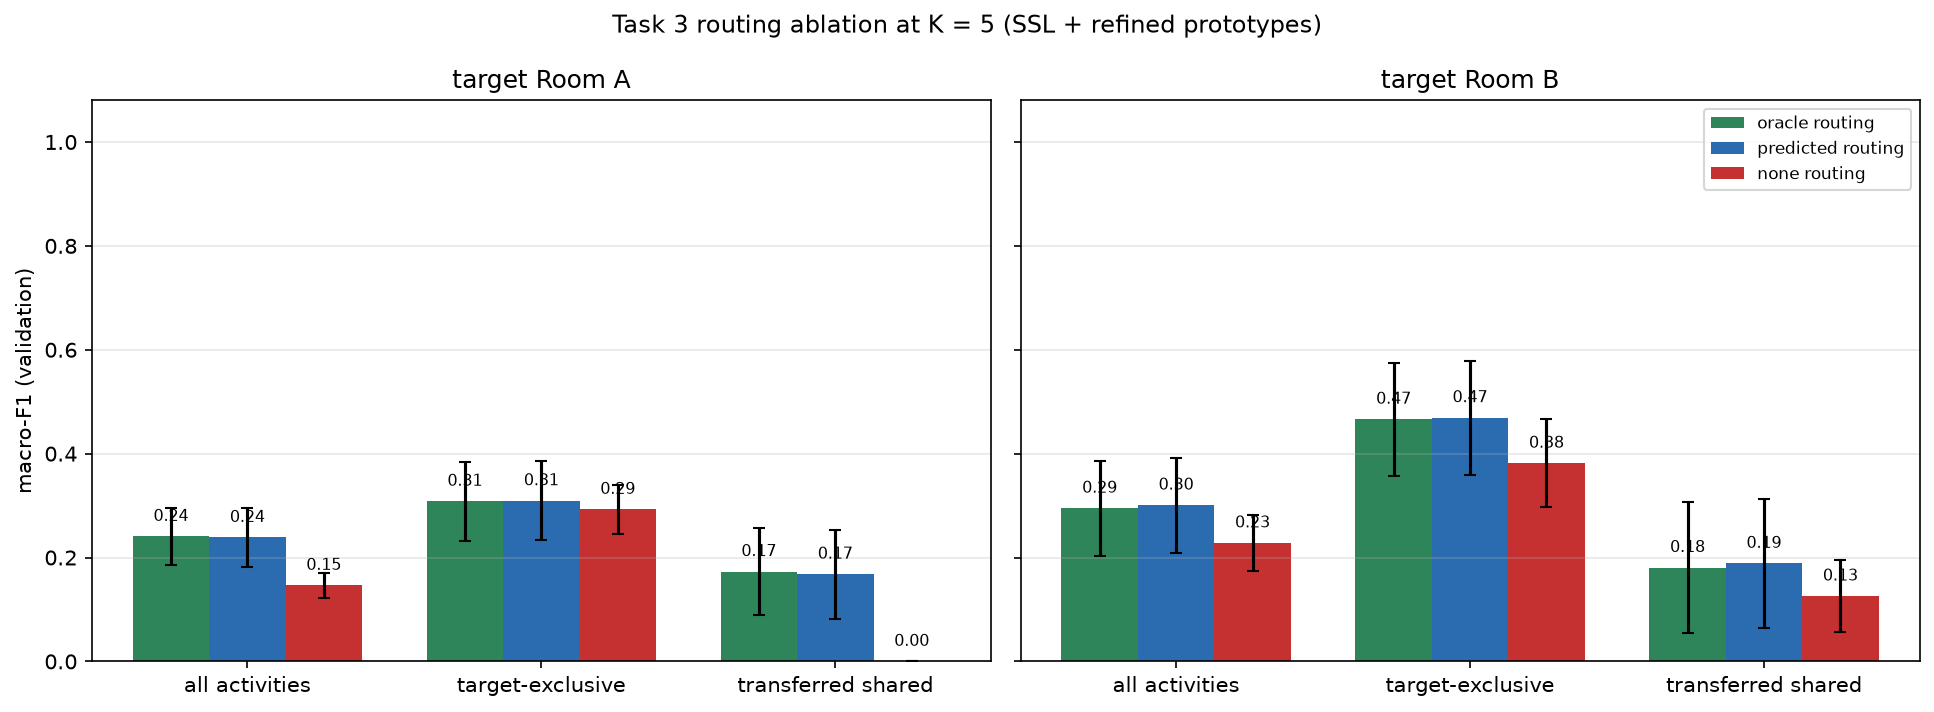
\includegraphics[width=0.44\linewidth]{figures/task3_routing.png}
\caption{Routing ablation at $K=5$: oracle vs predicted vs no routing, both target rooms.}
\label{fig:task3_routing}
\end{figure}

Predicted routing matches oracle routing to within $\mathbf{0.006}$ F1 ($0.240$ vs $0.240$ in Room~A; $0.343$ vs $0.337$ in Room~B), while removing routing costs $6.0$ points in Room~A ($0.240 \to 0.180$) and $\mathbf{14.2}$ in Room~B ($0.337 \to 0.195$), because target windows are then absorbed by source-exclusive prototypes that cannot apply (Room~B windows predicted \textsc{Fall}). Routing protects the decision boundary --- but since Task~1 succeeds on session artifacts, routing is close to free here and the oracle-versus-predicted gap is the only informative comparison.

% =========================================================================
\section{Critical Limitations \& Confounding Factors}
% =========================================================================
In accordance with Section~12 of the challenge specification, we explicitly document six structural limitations of the benchmark:
\begin{enumerate}
    \item \textbf{Room vs session (§12.1):} the two rooms were recorded in disjoint sessions, so any classifier also keys on oscillator drift, interference and transmission timing.
    \item \textbf{Activity vs location (§12.2):} Room~A activities were performed in fixed spatial sub-regions, so multipath fading correlates with the label.
    \item \textbf{Two-room horizon (§12.3):} only $\mathcal{A} \leftrightarrow \mathcal{B}$ transfer is measured; generalisation to an unseen room is not established.
    \item \textbf{Capture- not subject-disjoint (§12.4):} subjects overlap across splits, so subject-independent generalisation is untested.
    \item \textbf{Not comparable to the original paper (§12.5):} its random 80/20 split leaks capture-level correlation; ours is capture-disjoint.
    \item \textbf{Archive asymmetry (§12.6):} Experiment~2 is raw PCAP and Experiment~3 pre-extracted CSV, an upstream instrumentation difference we cannot remove.
\end{enumerate}

% =========================================================================
\section{Team Member Contributions \& Logistics}
% =========================================================================
The project was executed by Team Klique under a modular, test-driven engineering structure. Table~\ref{tab:contributions} summarizes individual technical contributions.

\begin{table}[htbp]
\centering
\footnotesize
\setlength{\tabcolsep}{4pt}
\caption{Team Member Contribution Statement.}
\label{tab:contributions}
\begin{tabular}{p{0.24\textwidth}p{0.70\textwidth}}
\toprule
\textbf{Team Member} & \textbf{Core Technical Contributions \& Responsibilities} \\
\midrule
\textbf{R Mohan Poornachandra} \newline (23EX10027) & \textbf{Track 1 --- ingestion, normalisation, Task 1:} clean-room PCAP parser and empirical BCM4366c0 bitfield resolution (\texttt{pcap\_reader.py}, \texttt{csi\_decode.py}); discovery of the Nexmon frame-interleaving artifact; deterministic windowing and manifest provenance (\texttt{windowing.py}); leakage-safe normalisation presets (\texttt{normalization.py}); Task~1 ablation ladder and session-confound analysis; the Room~B \textsc{Walk} amplitude-shortcut diagnosis, the \texttt{per\_window\_scalar} scope behind \texttt{task2\_level\_free}, and the Hungarian assignment diagnostic (\texttt{task3\_diagnostics.py}); technical report. \\
\midrule
\textbf{Hemant} \newline (22CS30029) & \textbf{Track 2 --- representation learning:} 1D dilated residual CNN backbone (\texttt{encoder.py}); SimCLR/NT-Xent pretraining (\texttt{ssl\_pretrain.py}); adjacency-breaking augmentations; 416-d handcrafted and random-weight baselines (\texttt{baselines.py}); frozen linear-probe cross-validation (\texttt{task2\_probe.py}); UMAP diagnostics. \\
\midrule
\textbf{Saras Wagh} \newline (22CS30048) & \textbf{Track 3 --- few-shot adaptation:} prototypical networks and soft $k$-means refinement (\texttt{fewshot.py}); capture-level support sampling and the $K$-sweep driver (\texttt{task3\_adapt.py}); executed the full \texttt{task2\_level\_free} programme --- encoder retraining and the complete Task~3 rerun on which all results in Sections~5--6 are based --- and authored the retraction in Section~6.2; integrated the Hungarian diagnostic; routing ablation; confusion and label-efficiency figures. \\
\bottomrule
\end{tabular}
\end{table}

\noindent\textbf{Teaching Team Repository Access:} Collaborator access to the GitHub repository has been granted to the course instructors: \texttt{sandipc-iitkgp}, \texttt{sayantan-kuila}, and \texttt{debjit2001}.

% =========================================================================
\section{Mandatory AI Tool Use Disclosure}
% =========================================================================
In compliance with the CS60055 academic integrity policy we disclose AI assistance in full, including
cases where it was substantial rather than incidental.

\noindent\textbf{Tools used.} Anthropic Claude, driven interactively through Claude Code as an agentic
pair-programming assistant with repository and shell access. All three members used this same assistant;
no other AI tool was used on any part of this project.

\noindent\textbf{Substantial assistance (Track 1: ingestion, normalisation, Task 1 and diagnostics).}
Working from the author's direction in extended interactive sessions, the assistant produced first-draft
implementations of every module in the ingestion, quality-control, windowing, normalisation, Task~1 and
diagnostics tracks (\texttt{pcap\_reader}, \texttt{csi\_decode}, \texttt{amplitude}, \texttt{csv\_reader},
\texttt{cleaning}, \texttt{windowing}, \texttt{splits}, \texttt{normalization}, \texttt{dataset},
\texttt{config}, \texttt{task1\_room}, \texttt{task1\_ablation}, \texttt{task3\_diagnostics}), the
leakage test suite, \texttt{run\_episode.py}, \texttt{configs/experiment.yaml}, the repository
documentation and Figure~\ref{fig:pipeline_diagram}.
Three findings reported in this paper also first surfaced during those sessions and were then reproduced
and confirmed by the team: the empirical packed-CSI bitfield resolution (Section~2.2), the Nexmon
frame-interleaving artifact and its consequence for the 150-observation window (Section~2.3), and the
Room~B \textsc{Walk} amplitude shortcut that forced the \texttt{task2\_level\_free} retraction
(Section~6.2). The \texttt{per\_window\_scalar} normalisation scope introduced to remove that shortcut was
likewise drafted with the assistant; the encoder retraining and the full Task~3 rerun on the resulting
representation were carried out by the team.

\noindent\textbf{Routine assistance.} Debugging bitwise sign extension, pytest boilerplate, Matplotlib and
\LaTeX{} layout, and prose editing of this report, including verifying every reported number against the
committed \texttt{results/*.csv} files.

\noindent\textbf{Track 2 and Track 3 model code} (\texttt{encoder.py}, \texttt{ssl\_pretrain.py},
\texttt{baselines.py}, \texttt{task2\_probe.py}, \texttt{fewshot.py}, \texttt{task3\_adapt.py}) was written by
the members credited in Table~\ref{tab:contributions} using the same assistant in the same capacity:
AI-drafted implementations followed by author review, execution and verification. The design decisions
those files embody --- the encoder topology, the NT-Xent objective and its temperature, the
adjacency-breaking augmentation set, the handcrafted feature basis, the prototype and soft $k$-means
formulations, the support-sampling protocol and the routing ablation --- were made by those authors, who
also ran every experiment reported from them.

\noindent\textbf{Author responsibility.} No AI-generated component was accepted without review. Every
design decision, every rejected alternative and every claim in this report was checked by the responsible
author against data the team regenerated; each member can explain the purpose and behaviour of every stage
they are credited with, as Section~6 of the specification requires.

% =========================================================================
\section{Conclusion}
% =========================================================================
We engineered an independent, clean-room Python pipeline for cross-room WiFi activity recognition, and showed that both naive environment recognition and few-shot activity transfer are confounded by acquisition artifacts: Nexmon frame interleaving, software amplitude scaling and class-level loudness offsets. A 1D dilated residual CNN pretrained by SimCLR with adjacency-breaking augmentations reaches an 8-class Macro-F1 of $\mathbf{0.924 \pm 0.013}$, exceeding handcrafted kinematic features ($0.893$) and random weights ($0.616$). Prototypical networks learn novel target-exclusive activities from very few labels ($\text{F1} \approx 0.59$ at $K=20$), but unlabelled shared-activity transfer fails through multipath-induced kinematic swaps. Cross-room WiFi sensing therefore requires active spatial-multipath calibration, not representation learning alone.

% =========================================================================
% References
% =========================================================================
\bibliographystyle{IEEEtran}
\begin{multicols}{2}
\scriptsize
\begin{thebibliography}{10}
\setlength{\itemsep}{1pt}
\setlength{\parskip}{0pt}

\bibitem{csi_dataset}
IEEE DataPort, ``CSI Human Activity Dataset,'' 2021. \url{https://ieee-dataport.org/open-access/csi-human-activity}.

\bibitem{schafer2021human}
J.~Sch{\"a}fer, B.~R. Barrsiwal, M.~Kokhkharova, H.~Adil, and J.~Liebehenschel, ``Human Activity Recognition Using CSI Information with Nexmon,'' \emph{Applied Sciences}, vol.~11, no.~19, p. 8860, 2021.

\bibitem{gringoli2019free}
F.~Gringoli \emph{et~al.}, ``Free Your CSI: A CSI Extraction Platform for Modern Wi-Fi Chipsets,'' in \emph{Proc. ACM WiNTECH}, 2019, pp. 21--28.

\bibitem{chen2020simple}
T.~Chen, S.~Kornblith, M.~Norouzi, and G.~Hinton, ``A Simple Framework for Contrastive Learning of Visual Representations,'' in \emph{Proc. ICML}, 2020, pp. 1597--1607.

\bibitem{snell2017prototypical}
J.~Snell, K.~Swersky, and R.~Zemel, ``Prototypical Networks for Few-shot Learning,'' in \emph{Proc. NeurIPS}, vol.~30, 2017.

\bibitem{wang2015understanding}
H.~Wang \emph{et~al.}, ``Human Respiration Detection with Commodity WiFi Devices,'' in \emph{Proc. ACM UbiComp}, 2015, pp. 25--36.

\bibitem{yang2018device}
J.~Yang \emph{et~al.}, ``Device-Free Human Activity Recognition Using Handheld Devices,'' \emph{IEEE IoT J.}, vol.~5, no.~2, pp. 796--805, 2018.

\bibitem{li2019towards}
H.~Li \emph{et~al.}, ``Wi-Motion: Robust Human Activity Recognition Using WiFi Signals,'' \emph{IEEE IoT J.}, vol.~6, no.~4, pp. 6934--6946, 2019.

\bibitem{pedregosa2011scikit}
F.~Pedregosa \emph{et~al.}, ``Scikit-learn: Machine Learning in Python,'' \emph{Journal of Machine Learning Research}, vol.~12, pp. 2825--2830, 2011.

\bibitem{paszke2019pytorch}
A.~Paszke \emph{et~al.}, ``PyTorch: An Imperative Style, High-Performance Deep Learning Library,'' in \emph{Proc. NeurIPS}, vol.~32, 2019.

\end{thebibliography}
\end{multicols}

\end{document}
